


As a setting to illustrate computer techniques for describing variability, take
the data that Galton collected on the heights of adult children
and their parents. \datasetGalton
The file \texttt{galton.csv} stores these data in a modern,
case/variable format.

\begin{Schunk}
\begin{Sinput}
> require(mosaic)
> galton = fetchData("galton.csv")
\end{Sinput}
\end{Schunk}

\subsection{Simple Statistical Calculations}

\index{C}{descriptive statistics!computing|(}

Simple numerical descriptions are easy to compute.  Here are the mean,
median, standard deviation and variance of the children's heights (in
inches).
\index{P}{Descriptive Statistics!mean@\texttt{mean}}
\index{P}{Descriptive Statistics!sd@\texttt{sd}}
\index{P}{Descriptive Statistics!median@\texttt{median}}
\index{P}{mean@\texttt{mean}}
\index{P}{median@\texttt{median}}
\index{P}{sd@\texttt{sd}}
\index{P}{var@\texttt{var}}
\index{C}{variance!sqrt of standard deviation}
\begin{Schunk}
\begin{Sinput}
> mean(height, data=galton)
\end{Sinput}
\begin{Soutput}
[1] 66.8
\end{Soutput}
\begin{Sinput}
> median(height, data=galton)
\end{Sinput}
\begin{Soutput}
[1] 66.5
\end{Soutput}
\begin{Sinput}
> sd(height, data=galton)
\end{Sinput}
\begin{Soutput}
[1] 3.58
\end{Soutput}
\begin{Sinput}
> var(height, data=galton)
\end{Sinput}
\begin{Soutput}
[1] 12.8
\end{Soutput}
\end{Schunk}

Notice that the variance function (\function{var}) returns the square
of the standard deviation (\function{sd}).
Having both is merely a convenience.

\index{P}{Descriptive Statistics!pdata@\texttt{pdata}}
\index{P}{Descriptive Statistics!qdata@\texttt{qdata}}
\index{C}{percentile!quantile operator}
\index{P}{quantile@\texttt{quantile}}
\index{P}{qdata@\texttt{qdata}*}
\index{P}{pdata@\texttt{pdata}*}
A percentile tells where a given value falls in a distribution.  For example, a height of 63 inches is on the short side in Galton's data:
\begin{Schunk}
\begin{Sinput}
> pdata(63, height, data=galton)
\end{Sinput}
\begin{Soutput}
[1] 0.192
\end{Soutput}
\end{Schunk}
Only about 19\% of the cases have a height less than or equal to 63 inches.  The \code{pdata} operator takes one or more values as a first argument and finds where they fall in the distribution of values in the second argument.

A quantile refers to the same sort of calculation, but inverted.  Instead of giving a value in the same units as the distribution, you give a probability: a number between 0 and 1.  The \code{qdata} operator then calculates the value whose percentile would be that value:
\begin{Schunk}
\begin{Sinput}
> qdata(0.20, height, data=galton)
\end{Sinput}
\begin{Soutput}
 20% 
63.5 
\end{Soutput}
\end{Schunk}
Remember that the probability is given as a number between 0 and 1, so use 0.50 to indicate that you want the value which falls at the 50th percentile.

\begin{itemize}
\index{C}{quantiles!and coverage intervals}
\index{C}{coverage interval!quantiles}
\item The 25th and 75th percentile in a single command --- in other
  words, the 50 percent coverage interval:
\begin{Schunk}
\begin{Sinput}
> qdata(c(0.25, 0.75), height, data=galton)
\end{Sinput}
\begin{Soutput}
 25%  75% 
64.0 69.7 
\end{Soutput}
\end{Schunk}

\item The 2.5th and 97.5th percentile --- in other words, the 95
  percent coverage interval:
\begin{Schunk}
\begin{Sinput}
> qdata(c(0.025, 0.975), height, data=galton)
\end{Sinput}
\begin{Soutput}
 2.5% 97.5% 
   60    73 
\end{Soutput}
\end{Schunk}
\end{itemize}

The interquartile range is the width of the 50 percent coverage
interval:
\begin{Schunk}
\begin{Sinput}
> IQR(height, data=galton)
\end{Sinput}
\begin{Soutput}
[1] 5.7
\end{Soutput}
\end{Schunk}

Some other useful operators are \function{min}, \function{max}, and
\function{range}.  
\index{P}{min@\texttt{min}}
\index{P}{max@\texttt{max}}
\index{P}{range@\texttt{range}}

\index{C}{descriptive statistics!computing|)}


\subsection{Simple Statistical Graphics}

\index{C}{graphics!statistical|(}
\index{C}{statistical graphics|(}
There are several basic types of statistical graphics to display
the distribution of a variable: histograms, density plots, and
boxplots.  These are easily mastered by example. 

\subsubsection{Histograms and Distributions}

\index{C}{histogram!drawing}
\index{P}{histogram@\texttt{histogram}}
\index{P}{Plotting \& Graphics!histogram@\texttt{histogram}}

Constructing a histogram involves dividing the range of a variable up
into bins and counting how many cases fall into each bin.  This is
done in an almost entirely automatic way:
\begin{Schunk}
\begin{Sinput}
> histogram( galton$height )
\end{Sinput}
\end{Schunk}
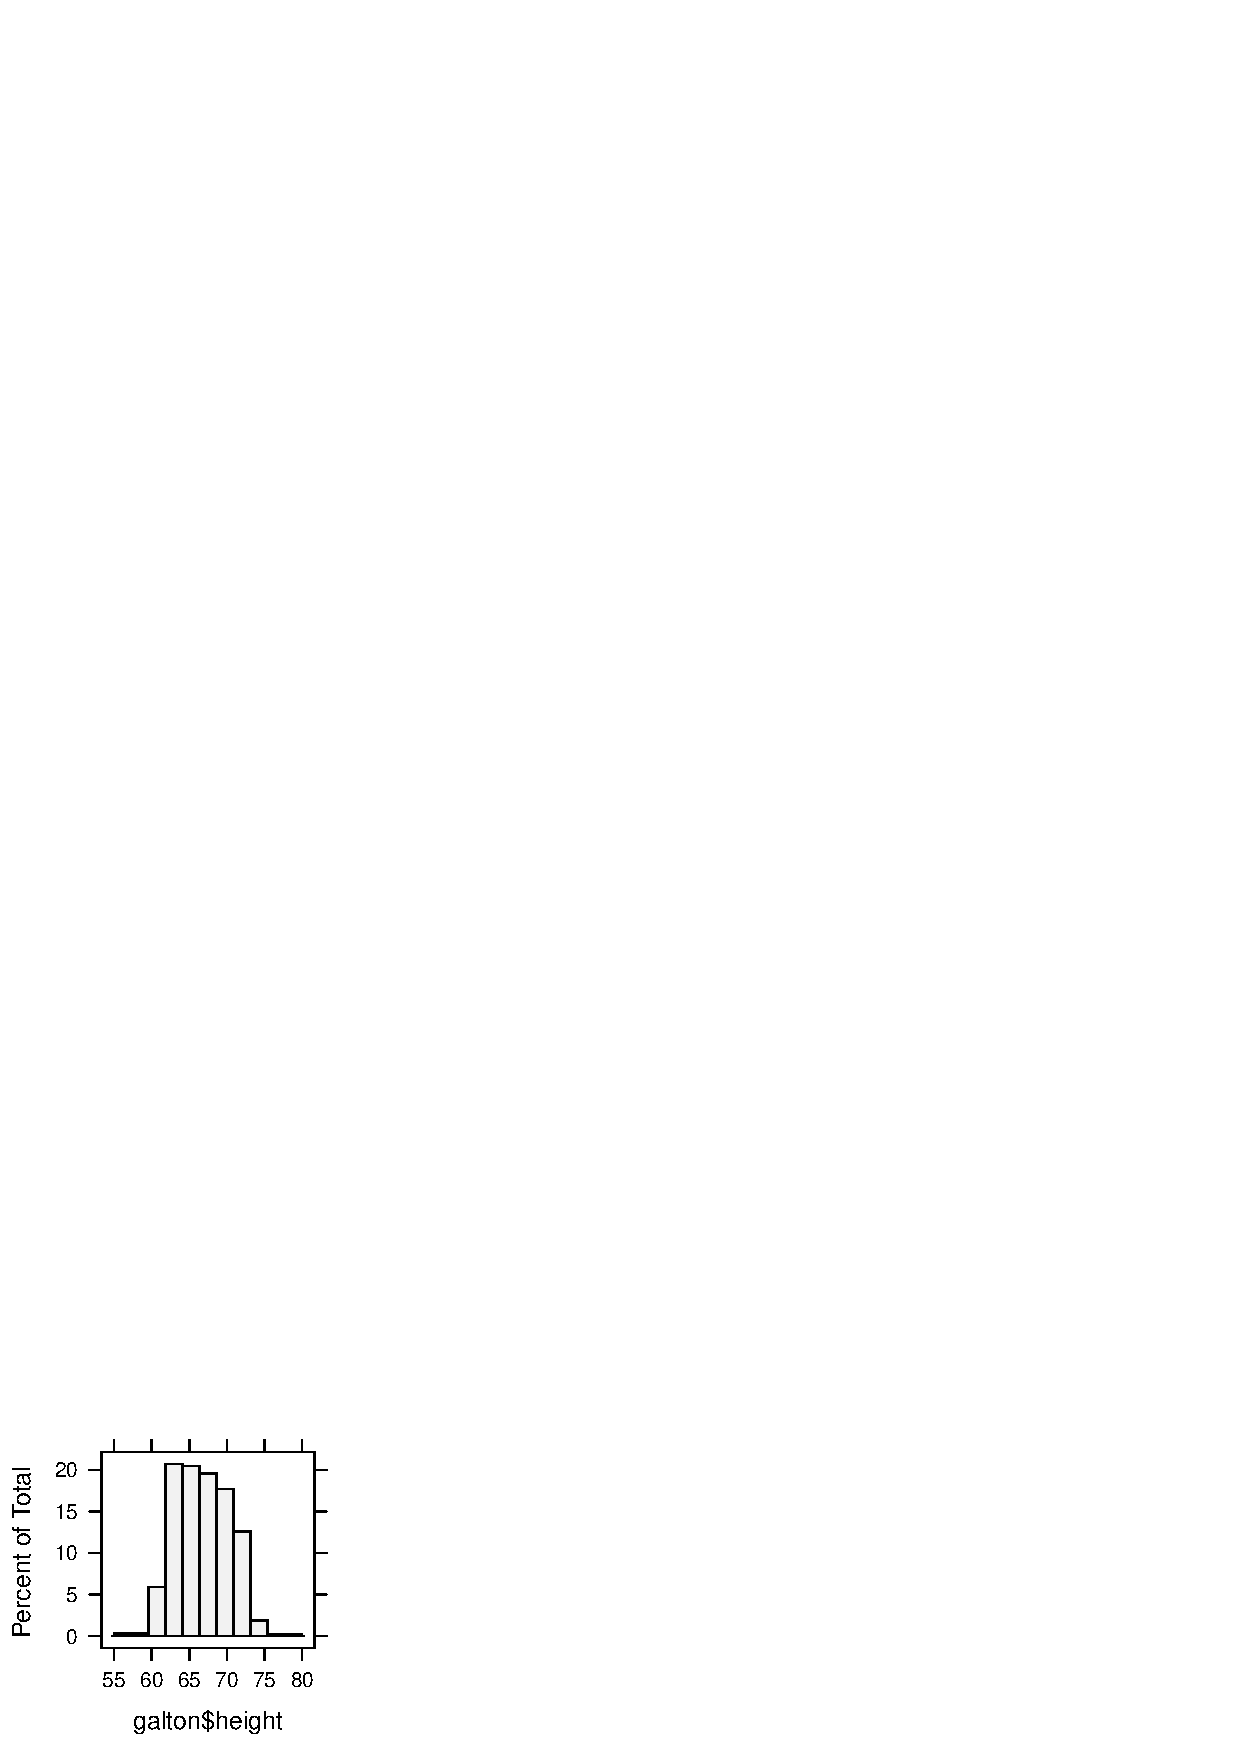
\includegraphics{Figures/variation-var1-hist}

When constructing a histogram, R makes an automatic but sensible
choice of the number of bins.  If you like, you can control this
yourself.  For instance:
\begin{Schunk}
\begin{Sinput}
> histogram( galton$height, breaks=25 )
\end{Sinput}
\end{Schunk}
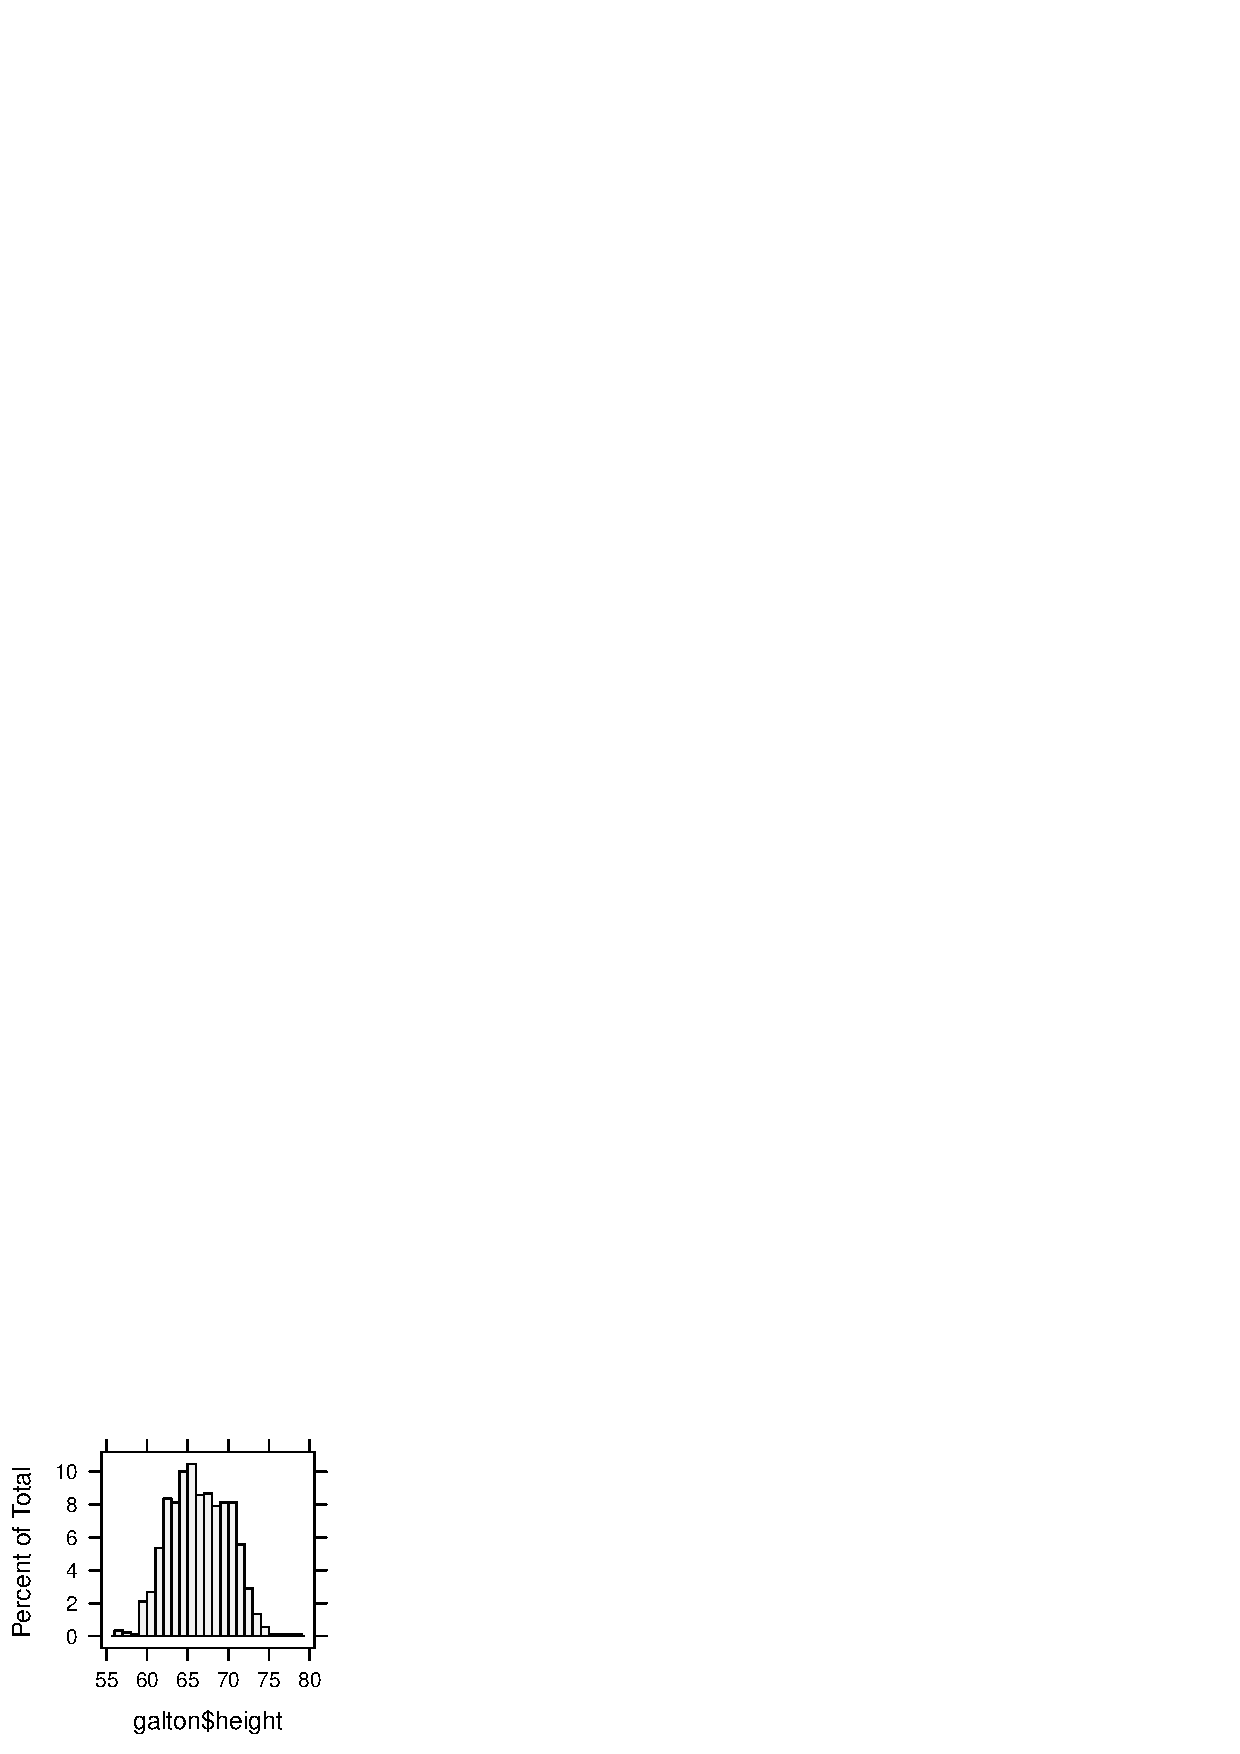
\includegraphics{Figures/variation-var2-hist}

The  horizontal axis of the histogram is always in the units of the variable.
For the histograms above, the  horizontal axis is in ``inches'' because that
is the unit of the \code{galton$height} variable.       % $

The vertical axis is conventionally drawn in one of three ways:
controlled by an optional argument named \code{type}.
\begin{description}
\item[Absolute Frequency or Counts]  A simple count of the number of cases that
  falls into each bin.  This mode is set with
  \code{type="count"} as in 
\begin{Schunk}
\begin{Sinput}
> histogram( galton$height, type="count")
\end{Sinput}
\end{Schunk}
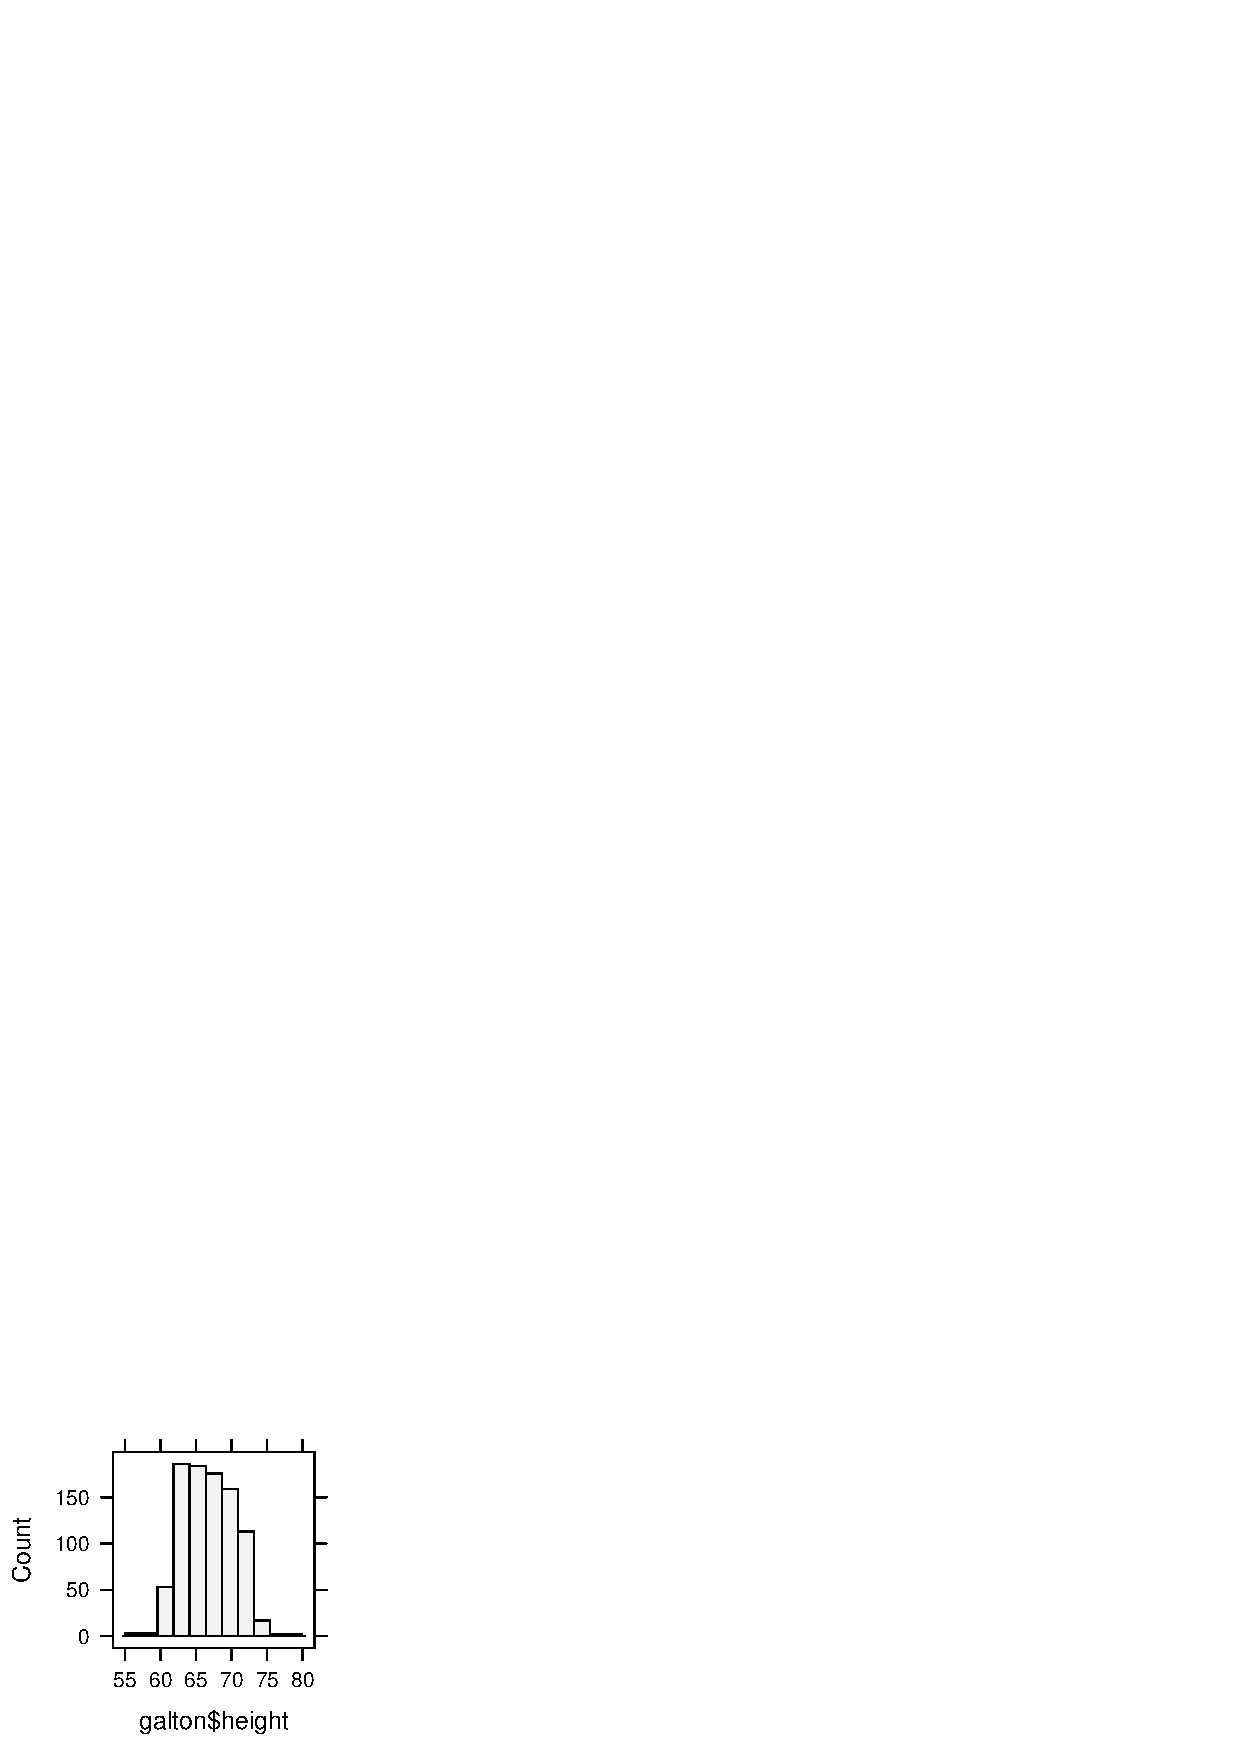
\includegraphics{Figures/variation-var3-hist}

\item[Relative Frequency] The vertical axis is scaled so that the 
height of the bar give the proportion of cases that fall into the
bin.  This is the default.
\item[Density] The vertical axis 
{\em area} of the bar gives the relative proportion of cases that fall
into the bin.  Set \code{type="density"} as in \code{histogram(galton$height,type="density")} .   % $ -kill the math mode
\end{description}
In a density plot, areas can be interpreted as probabilities and the
area under the entire histogram is equal to 1.

Other useful optional arguments set the labels for the axes and the
graph as a whole and color the bars.  For example,
\begin{Schunk}
\begin{Sinput}
> histogram(galton$height, type="density",
     xlab="Height (inches)", 
     main="Distribution of Heights",
     col="gray")
\end{Sinput}
\end{Schunk}
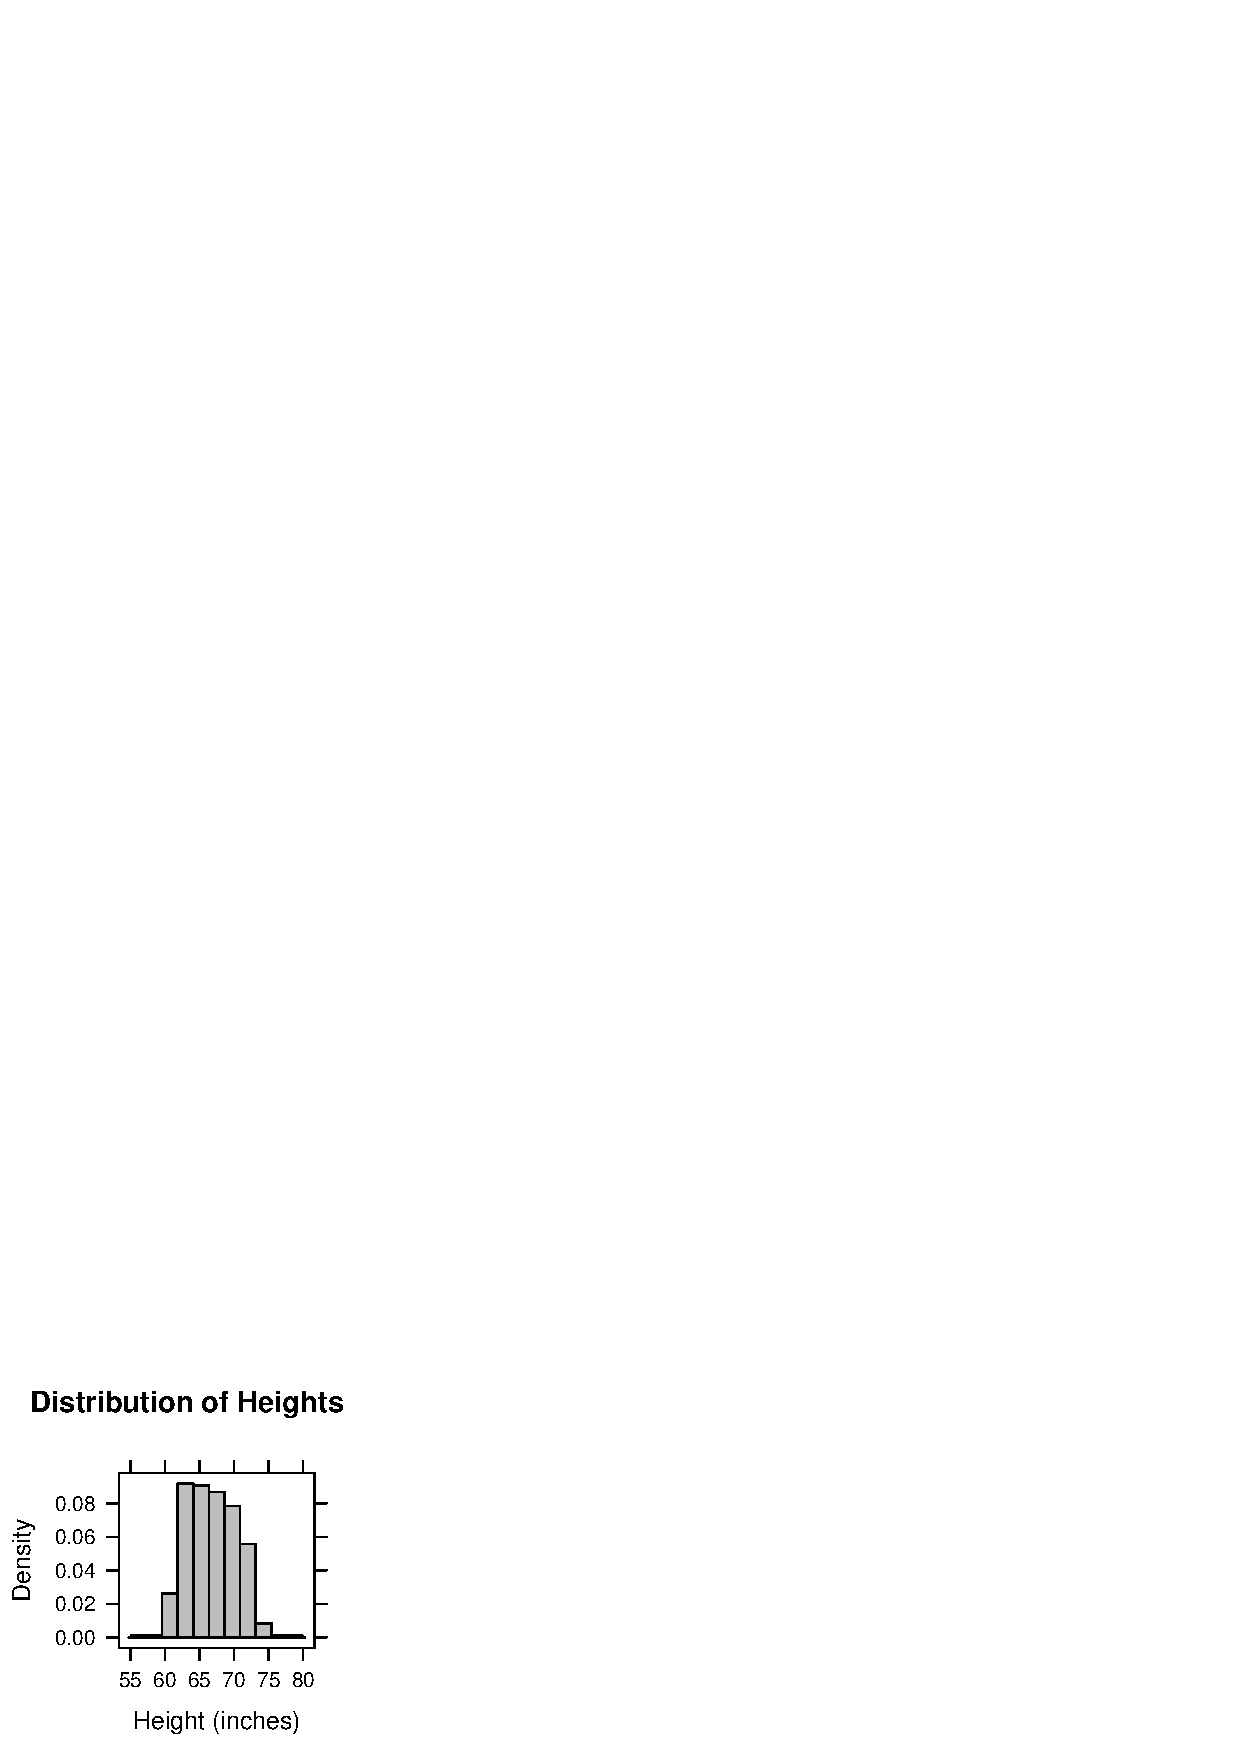
\includegraphics{Figures/variation-var4-hist}

The above command is so long that it has been broken into several
lines for display purposes.  R ignores the line breaks, holding off on
executing the command until it sees the final closing parentheses.
Notice the use of quotation marks to delimit the labels and names like
\code{"blue"}.

\subsubsection{Density Plots}

\index{P}{densityplot@\texttt{densityplot}}
\index{P}{Plotting \& Graphics!densityplot@\texttt{densityplot}}

\index{C}{density plot!drawing}
A \newword{density plot} avoids the need to create bins and plots out
the distribution as a continuous curve.  Making a density plot
involves two operators.  The \newword{density} operator performs the
basic computation which is then displayed using either the \code{plot}
or the \code{lines} operator.  For example:
\begin{Schunk}
\begin{Sinput}
> densityplot(galton$height) 
\end{Sinput}
\end{Schunk}
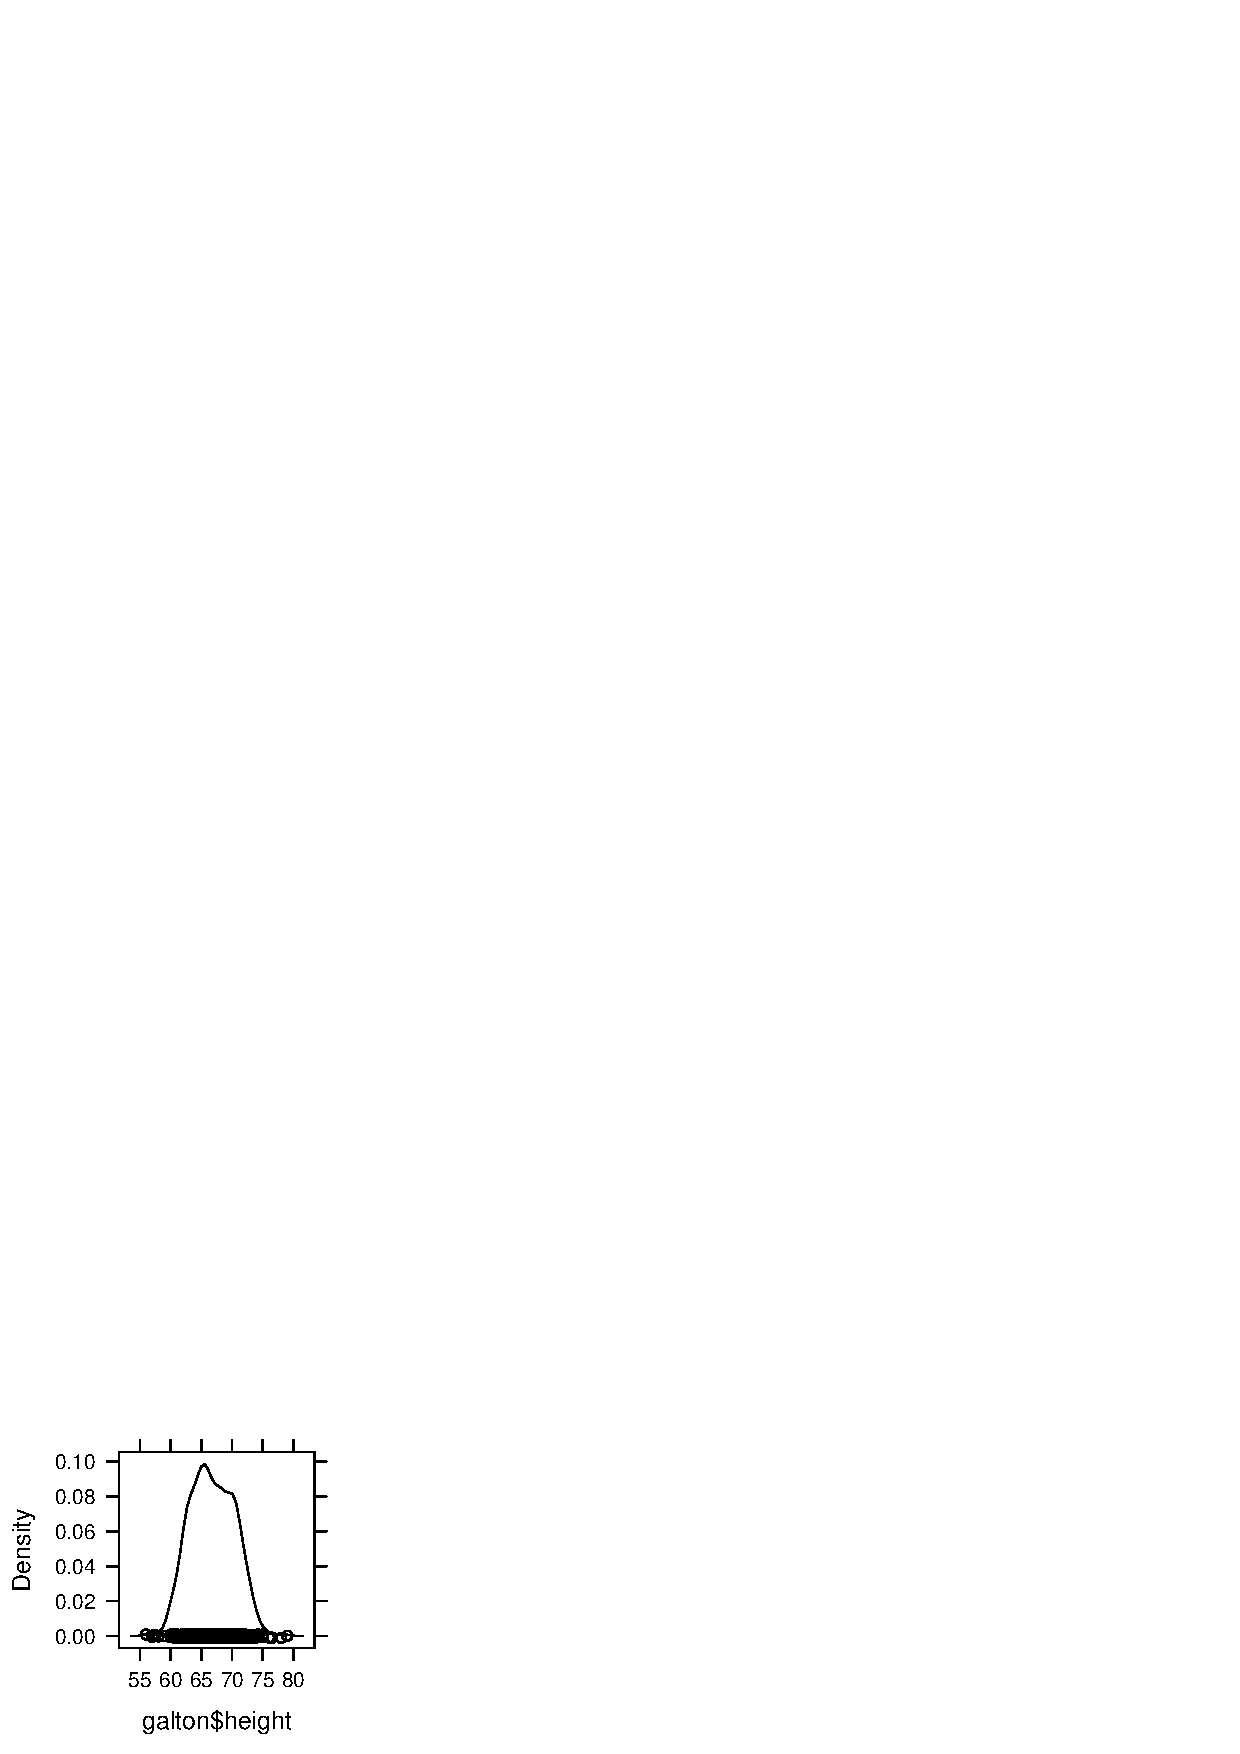
\includegraphics{Figures/variation-var5-density}

If you want to suppress the rug-like plotting of points at the bottom
of the graph, use \code{densityplot(galton$height,plot.points=FALSE)}. % $

\subsubsection{Box-and-Whisker Plots}

Box-and-whisker plots are made with the \code{bwplot} command:
\begin{Schunk}
\begin{Sinput}
> bwplot(galton$height)
\end{Sinput}
\end{Schunk}
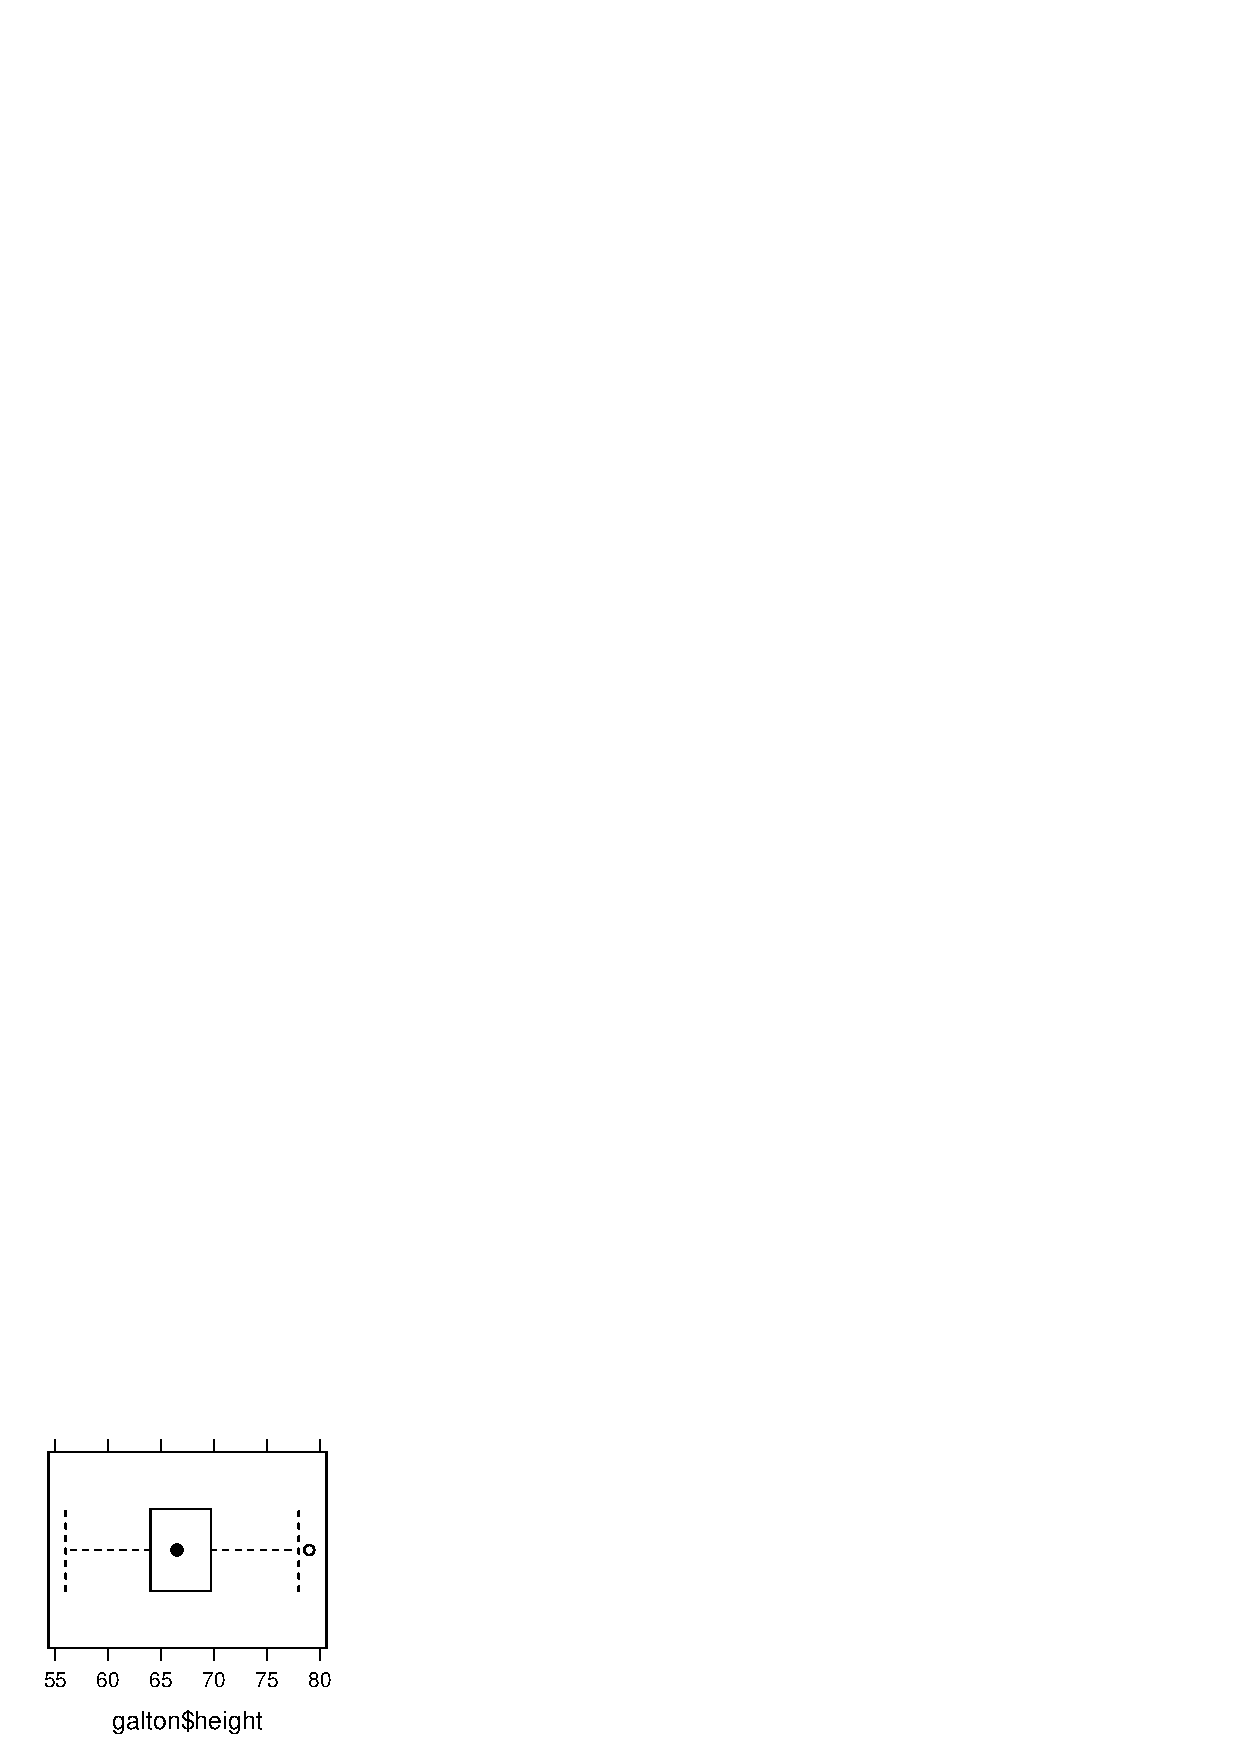
\includegraphics{Figures/variation-var6-bw}

The median is represented by the heavy dot in the middle.  Outliers,
if any, are marked by dots outside the whiskers.
\index{C}{outlier!in box plots}
\index{C}{box plot!outliers}

\index{C}{box plot!drawing}
\index{P}{bwplot@\texttt{bwplot}}
\index{P}{Plotting \& Graphics!bwplot@\texttt{bwplot}}
\index{C}{box and whisker plots|see{box plots}}
The real power of the box-and-whisker plot is for comparing
distributions.  This will be raised again more systematically in later
chapters, but just to illustrate, here is how to compare the heights
of males and females:

\begin{Schunk}
\begin{Sinput}
> bwplot(height ~ sex, data=galton)
\end{Sinput}
\end{Schunk}
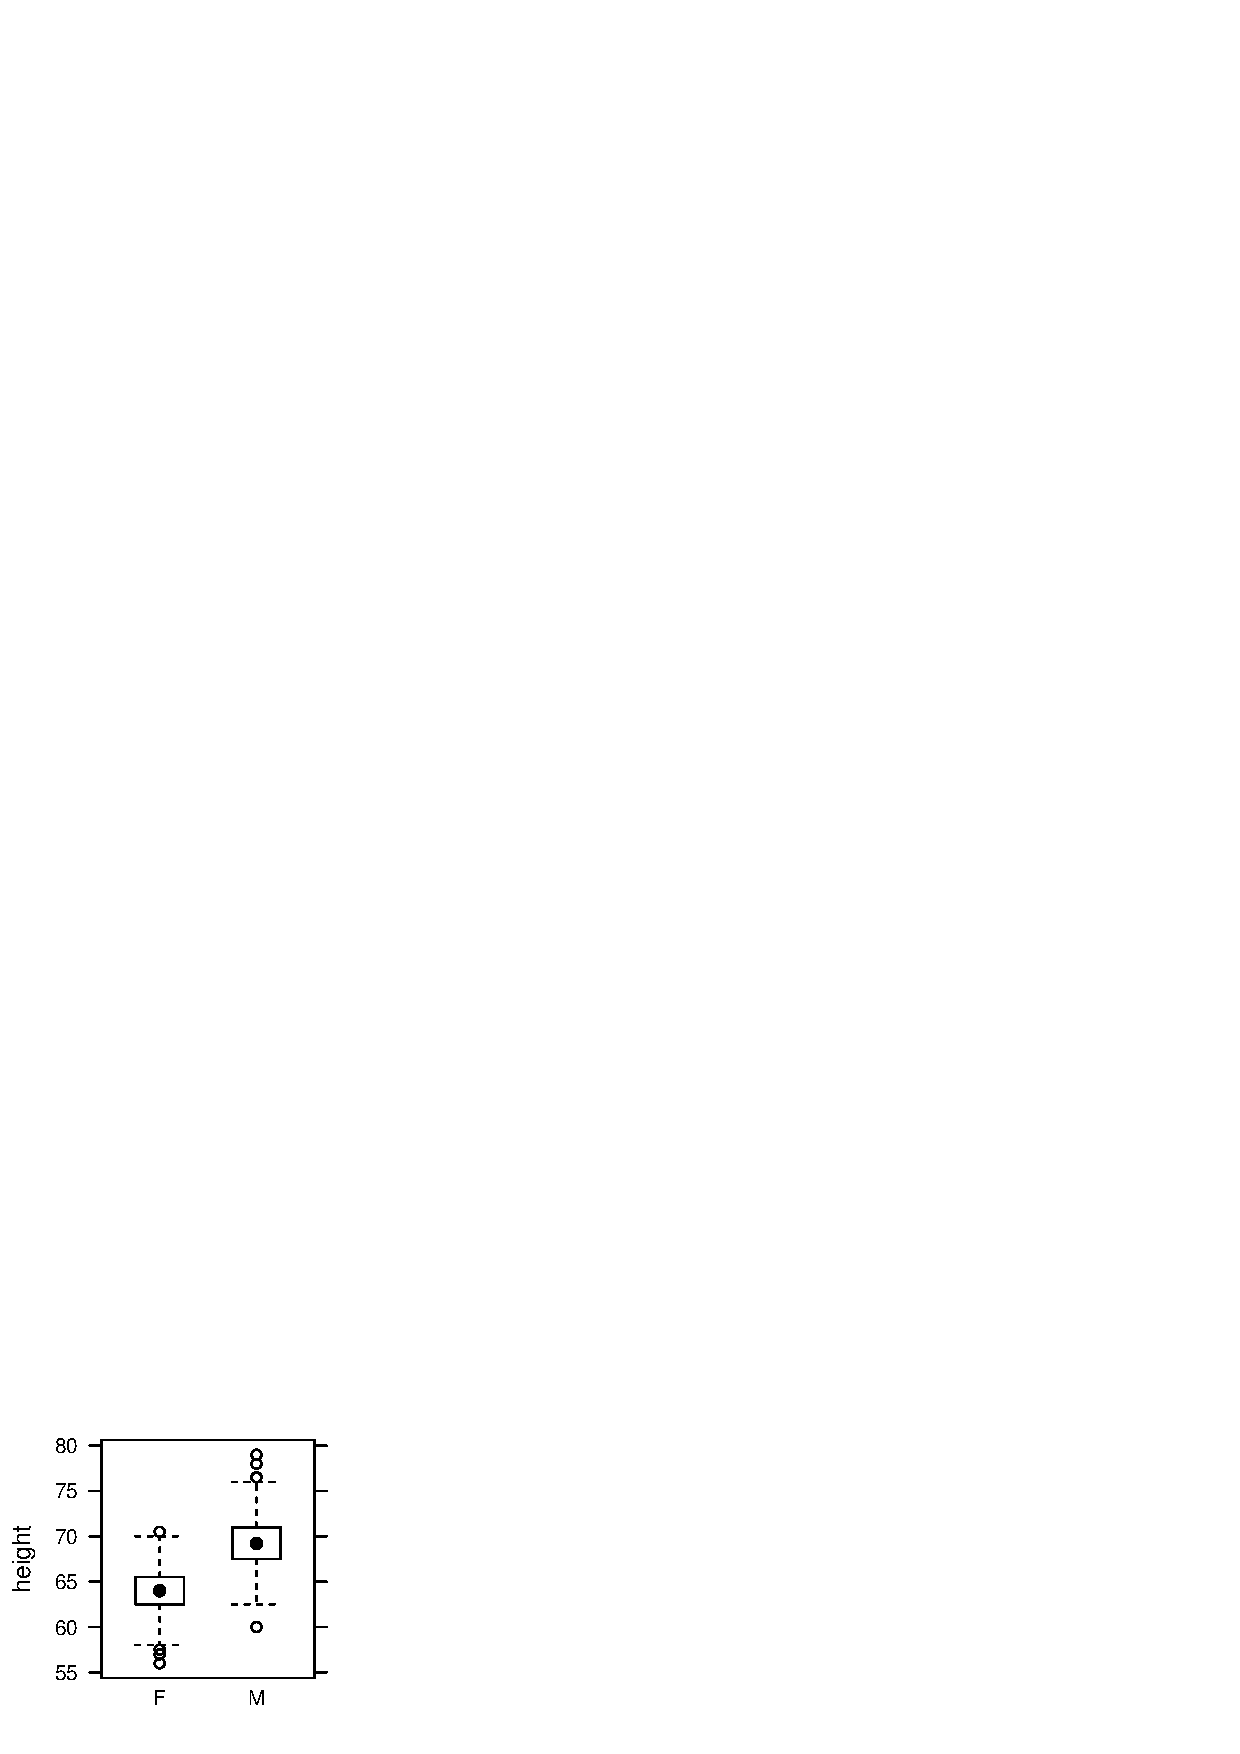
\includegraphics{Figures/variation-var7-bw}

\subsection{Displays of Categorical Variables}

\index{C}{counts!computing}
\index{C}{proportions!computing}
\index{P}{counts@\texttt{counts}}
\index{P}{props@\texttt{props}}
\index{P}{Descriptive Statistics!props@\texttt{props}}
\index{C}{table!of counts}
For categorical variables, it makes no sense to compute descriptive
statistics such as the mean, standard deviation, or variance.
Instead, look at the number of cases at each level of the variable.
\begin{Schunk}
\begin{Sinput}
> counts(sex, data=galton)
\end{Sinput}
\begin{Soutput}
  F   M 
433 465 
\end{Soutput}
\end{Schunk}
Proportions can be found in a similar way:
\begin{Schunk}
\begin{Sinput}
> props(sex, data=galton)
\end{Sinput}
\begin{Soutput}
    F     M 
0.482 0.518 
\end{Soutput}
\end{Schunk}


\index{C}{graphics!statistical|)}
\index{C}{statistical graphics|)}


